\documentclass[twoside]{book}

% Packages required by doxygen
\usepackage{fixltx2e}
\usepackage{calc}
\usepackage{doxygen}
\usepackage[export]{adjustbox} % also loads graphicx
\usepackage{graphicx}
\usepackage[utf8]{inputenc}
\usepackage{makeidx}
\usepackage{multicol}
\usepackage{multirow}
\PassOptionsToPackage{warn}{textcomp}
\usepackage{textcomp}
\usepackage[nointegrals]{wasysym}
\usepackage[table]{xcolor}

% Font selection
\usepackage[T1]{fontenc}
\usepackage[scaled=.90]{helvet}
\usepackage{courier}
\usepackage{amssymb}
\usepackage{sectsty}
\renewcommand{\familydefault}{\sfdefault}
\allsectionsfont{%
  \fontseries{bc}\selectfont%
  \color{darkgray}%
}
\renewcommand{\DoxyLabelFont}{%
  \fontseries{bc}\selectfont%
  \color{darkgray}%
}
\newcommand{\+}{\discretionary{\mbox{\scriptsize$\hookleftarrow$}}{}{}}

% Page & text layout
\usepackage{geometry}
\geometry{%
  a4paper,%
  top=2.5cm,%
  bottom=2.5cm,%
  left=2.5cm,%
  right=2.5cm%
}
\tolerance=750
\hfuzz=15pt
\hbadness=750
\setlength{\emergencystretch}{15pt}
\setlength{\parindent}{0cm}
\setlength{\parskip}{3ex plus 2ex minus 2ex}
\makeatletter
\renewcommand{\paragraph}{%
  \@startsection{paragraph}{4}{0ex}{-1.0ex}{1.0ex}{%
    \normalfont\normalsize\bfseries\SS@parafont%
  }%
}
\renewcommand{\subparagraph}{%
  \@startsection{subparagraph}{5}{0ex}{-1.0ex}{1.0ex}{%
    \normalfont\normalsize\bfseries\SS@subparafont%
  }%
}
\makeatother

% Headers & footers
\usepackage{fancyhdr}
\pagestyle{fancyplain}
\fancyhead[LE]{\fancyplain{}{\bfseries\thepage}}
\fancyhead[CE]{\fancyplain{}{}}
\fancyhead[RE]{\fancyplain{}{\bfseries\leftmark}}
\fancyhead[LO]{\fancyplain{}{\bfseries\rightmark}}
\fancyhead[CO]{\fancyplain{}{}}
\fancyhead[RO]{\fancyplain{}{\bfseries\thepage}}
\fancyfoot[LE]{\fancyplain{}{}}
\fancyfoot[CE]{\fancyplain{}{}}
\fancyfoot[RE]{\fancyplain{}{\bfseries\scriptsize Generated by Doxygen }}
\fancyfoot[LO]{\fancyplain{}{\bfseries\scriptsize Generated by Doxygen }}
\fancyfoot[CO]{\fancyplain{}{}}
\fancyfoot[RO]{\fancyplain{}{}}
\renewcommand{\footrulewidth}{0.4pt}
\renewcommand{\chaptermark}[1]{%
  \markboth{#1}{}%
}
\renewcommand{\sectionmark}[1]{%
  \markright{\thesection\ #1}%
}

% Indices & bibliography
\usepackage{natbib}
\usepackage[titles]{tocloft}
\setcounter{tocdepth}{3}
\setcounter{secnumdepth}{5}
\makeindex

% Hyperlinks (required, but should be loaded last)
\usepackage{ifpdf}
\ifpdf
  \usepackage[pdftex,pagebackref=true]{hyperref}
\else
  \usepackage[ps2pdf,pagebackref=true]{hyperref}
\fi
\hypersetup{%
  colorlinks=true,%
  linkcolor=blue,%
  citecolor=blue,%
  unicode%
}

% Custom commands
\newcommand{\clearemptydoublepage}{%
  \newpage{\pagestyle{empty}\cleardoublepage}%
}

\usepackage{caption}
\captionsetup{labelsep=space,justification=centering,font={bf},singlelinecheck=off,skip=4pt,position=top}

%===== C O N T E N T S =====

\begin{document}

% Titlepage & ToC
\hypersetup{pageanchor=false,
             bookmarksnumbered=true,
             pdfencoding=unicode
            }
\pagenumbering{roman}
\begin{titlepage}
\vspace*{7cm}
\begin{center}%
{\Large My Project }\\
\vspace*{1cm}
{\large Generated by Doxygen 1.8.11}\\
\end{center}
\end{titlepage}
\clearemptydoublepage
\tableofcontents
\clearemptydoublepage
\pagenumbering{arabic}
\hypersetup{pageanchor=true}

%--- Begin generated contents ---
\chapter{Class Index}
\section{Class List}
Here are the classes, structs, unions and interfaces with brief descriptions\+:\begin{DoxyCompactList}
\item\contentsline{section}{\hyperlink{structnode}{node} }{\pageref{structnode}}{}
\item\contentsline{section}{\hyperlink{structnode1}{node1} }{\pageref{structnode1}}{}
\item\contentsline{section}{\hyperlink{structnode__info}{node\+\_\+info} }{\pageref{structnode__info}}{}
\end{DoxyCompactList}

\chapter{File Index}
\section{File List}
Here is a list of all files with brief descriptions\+:\begin{DoxyCompactList}
\item\contentsline{section}{\hyperlink{Lab1_8c}{Lab1.\+c} }{\pageref{Lab1_8c}}{}
\end{DoxyCompactList}

\chapter{Class Documentation}
\hypertarget{structThreadParam}{}\section{Thread\+Param Struct Reference}
\label{structThreadParam}\index{Thread\+Param@{Thread\+Param}}
\subsection*{Public Attributes}
\begin{DoxyCompactItemize}
\item 
int $\ast$ \hyperlink{structThreadParam_aec444b4eb12a9a8fea3e8689e149c222}{array}
\item 
int \hyperlink{structThreadParam_a67d5841b5ec120d0265bc55eeb8bac6b}{value}
\item 
int \hyperlink{structThreadParam_a48b6fa880b0369abac96f8f54bf12e08}{start\+Index}
\item 
int \hyperlink{structThreadParam_a88bf854942e7037fbdd9269b434612d6}{end\+Index}
\end{DoxyCompactItemize}


\subsection{Member Data Documentation}
\index{Thread\+Param@{Thread\+Param}!array@{array}}
\index{array@{array}!Thread\+Param@{Thread\+Param}}
\subsubsection[{\texorpdfstring{array}{array}}]{\setlength{\rightskip}{0pt plus 5cm}int$\ast$ Thread\+Param\+::array}\hypertarget{structThreadParam_aec444b4eb12a9a8fea3e8689e149c222}{}\label{structThreadParam_aec444b4eb12a9a8fea3e8689e149c222}
\index{Thread\+Param@{Thread\+Param}!end\+Index@{end\+Index}}
\index{end\+Index@{end\+Index}!Thread\+Param@{Thread\+Param}}
\subsubsection[{\texorpdfstring{end\+Index}{endIndex}}]{\setlength{\rightskip}{0pt plus 5cm}int Thread\+Param\+::end\+Index}\hypertarget{structThreadParam_a88bf854942e7037fbdd9269b434612d6}{}\label{structThreadParam_a88bf854942e7037fbdd9269b434612d6}
\index{Thread\+Param@{Thread\+Param}!start\+Index@{start\+Index}}
\index{start\+Index@{start\+Index}!Thread\+Param@{Thread\+Param}}
\subsubsection[{\texorpdfstring{start\+Index}{startIndex}}]{\setlength{\rightskip}{0pt plus 5cm}int Thread\+Param\+::start\+Index}\hypertarget{structThreadParam_a48b6fa880b0369abac96f8f54bf12e08}{}\label{structThreadParam_a48b6fa880b0369abac96f8f54bf12e08}
\index{Thread\+Param@{Thread\+Param}!value@{value}}
\index{value@{value}!Thread\+Param@{Thread\+Param}}
\subsubsection[{\texorpdfstring{value}{value}}]{\setlength{\rightskip}{0pt plus 5cm}int Thread\+Param\+::value}\hypertarget{structThreadParam_a67d5841b5ec120d0265bc55eeb8bac6b}{}\label{structThreadParam_a67d5841b5ec120d0265bc55eeb8bac6b}


The documentation for this struct was generated from the following file\+:\begin{DoxyCompactItemize}
\item 
\hyperlink{Lab3_8cpp}{Lab3.\+cpp}\end{DoxyCompactItemize}

\hypertarget{structThreadReturn}{}\section{Thread\+Return Struct Reference}
\label{structThreadReturn}\index{Thread\+Return@{Thread\+Return}}
\subsection*{Public Attributes}
\begin{DoxyCompactItemize}
\item 
int \hyperlink{structThreadReturn_ada06b95a1d8c2688d8f7ff617ca82074}{count}
\item 
int \hyperlink{structThreadReturn_acee40ef3ef81baf05c35b71761d7ffad}{pos}
\end{DoxyCompactItemize}


\subsection{Member Data Documentation}
\index{Thread\+Return@{Thread\+Return}!count@{count}}
\index{count@{count}!Thread\+Return@{Thread\+Return}}
\subsubsection[{\texorpdfstring{count}{count}}]{\setlength{\rightskip}{0pt plus 5cm}int Thread\+Return\+::count}\hypertarget{structThreadReturn_ada06b95a1d8c2688d8f7ff617ca82074}{}\label{structThreadReturn_ada06b95a1d8c2688d8f7ff617ca82074}
\index{Thread\+Return@{Thread\+Return}!pos@{pos}}
\index{pos@{pos}!Thread\+Return@{Thread\+Return}}
\subsubsection[{\texorpdfstring{pos}{pos}}]{\setlength{\rightskip}{0pt plus 5cm}int Thread\+Return\+::pos}\hypertarget{structThreadReturn_acee40ef3ef81baf05c35b71761d7ffad}{}\label{structThreadReturn_acee40ef3ef81baf05c35b71761d7ffad}


The documentation for this struct was generated from the following file\+:\begin{DoxyCompactItemize}
\item 
\hyperlink{Lab3_8cpp}{Lab3.\+cpp}\end{DoxyCompactItemize}

\chapter{File Documentation}
\hypertarget{Lab3_8cpp}{}\section{Lab3.\+cpp File Reference}
\label{Lab3_8cpp}\index{Lab3.\+cpp@{Lab3.\+cpp}}
{\ttfamily \#include $<$iostream$>$}\\*
{\ttfamily \#include $<$pthread.\+h$>$}\\*
{\ttfamily \#include $<$stdio.\+h$>$}\\*
{\ttfamily \#include $<$stdlib.\+h$>$}\\*
{\ttfamily \#include $<$unistd.\+h$>$}\\*
Include dependency graph for Lab3.\+cpp\+:
\nopagebreak
\begin{figure}[H]
\begin{center}
\leavevmode
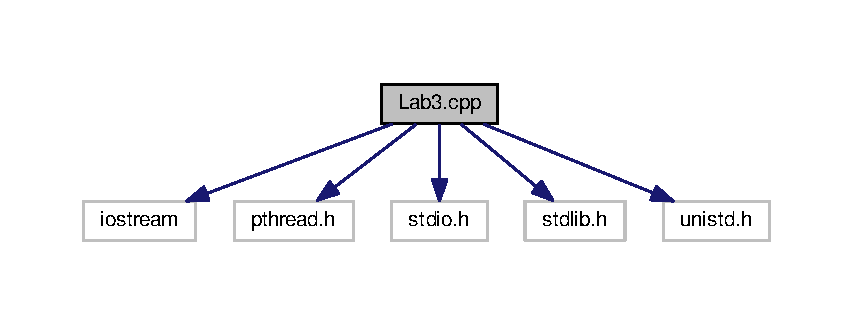
\includegraphics[width=350pt]{Lab3_8cpp__incl}
\end{center}
\end{figure}
\subsection*{Classes}
\begin{DoxyCompactItemize}
\item 
struct \hyperlink{structThreadReturn}{Thread\+Return}
\item 
struct \hyperlink{structThreadParam}{Thread\+Param}
\end{DoxyCompactItemize}
\subsection*{Functions}
\begin{DoxyCompactItemize}
\item 
void $\ast$ \hyperlink{Lab3_8cpp_a309dddc4f36d285135261c13128963c1}{Search} (void $\ast$arg)
\item 
int \hyperlink{Lab3_8cpp_a0ddf1224851353fc92bfbff6f499fa97}{main} (int argc, char $\ast$argv\mbox{[}$\,$\mbox{]})
\end{DoxyCompactItemize}


\subsection{Function Documentation}
\index{Lab3.\+cpp@{Lab3.\+cpp}!main@{main}}
\index{main@{main}!Lab3.\+cpp@{Lab3.\+cpp}}
\subsubsection[{\texorpdfstring{main(int argc, char $\ast$argv[])}{main(int argc, char *argv[])}}]{\setlength{\rightskip}{0pt plus 5cm}int main (
\begin{DoxyParamCaption}
\item[{int}]{argc, }
\item[{char $\ast$}]{argv\mbox{[}$\,$\mbox{]}}
\end{DoxyParamCaption}
)}\hypertarget{Lab3_8cpp_a0ddf1224851353fc92bfbff6f499fa97}{}\label{Lab3_8cpp_a0ddf1224851353fc92bfbff6f499fa97}

\begin{DoxyCode}
74 \{
75    pthread\_t * threads;
76    \hyperlink{structThreadParam}{ThreadParam} * threadsParams;
77 
78    \textcolor{keyword}{const} \textcolor{keywordtype}{int} MAX\_SIZE=10000;
79    \textcolor{keywordtype}{int} BigArray[MAX\_SIZE];
80 
81    \textcolor{keywordtype}{int} thread\_num;
82    \textcolor{keywordtype}{int} status, i;
83    \textcolor{keywordtype}{int} pos, value;
84 
85    \textcolor{comment}{//Todo: prepare the array to be sorted for                                                              
                                                                                                       }
86    \textcolor{comment}{// You can fill the array with random numbers (taking values in the range of 1...100)                   
                                                                                                       }
87 
88    \textcolor{keywordflow}{for}(\textcolor{keywordtype}{int} k=0; k<MAX\_SIZE; k++)
89    \{
90       BigArray[k] = rand()%200+1;
91    \}
92 
93    cout <<\textcolor{stringliteral}{"What values to search:"};
94    cin >> value;
95 
96    \textcolor{keywordflow}{do} \{
97       cout <<\textcolor{stringliteral}{"How many threads to create:"};
98       cin >> thread\_num;
99    \} \textcolor{keywordflow}{while} (thread\_num<=1);
100 
101    \textcolor{comment}{//threads = new pthread\_t[thread\_num]; //dynamically allocate the thread handler ...                    
                                                                                                       }
102    pthread\_t threads[thread\_num];
103 
104    \textcolor{comment}{//threadsParams = new ThreadParam[thread\_num];                                                          
                                                                                                       }
105    \hyperlink{structThreadParam}{ThreadParam} threadsParams[thread\_num];
106 
107    \textcolor{keywordtype}{int} increase = (MAX\_SIZE / thread\_num) - 1;
108    \textcolor{keywordtype}{int} start = 0;
109    \textcolor{keywordtype}{int} end = increase;
110 
111    \textcolor{keywordflow}{for} (i=0; i<thread\_num; i++)\{
112       \textcolor{comment}{//Todo: prepare the argument to be passed to i-th Search thread                                      
                                                                                                       }
113       \textcolor{comment}{//                                                                                                   
                                                                                                       }
114       threadsParams[i].\hyperlink{structThreadParam_a67d5841b5ec120d0265bc55eeb8bac6b}{value} = value;
115       threadsParams[i].\hyperlink{structThreadParam_a48b6fa880b0369abac96f8f54bf12e08}{startIndex} = start;
116       threadsParams[i].\hyperlink{structThreadParam_a88bf854942e7037fbdd9269b434612d6}{endIndex} = end;
117       threadsParams[i].\hyperlink{structThreadParam_aec444b4eb12a9a8fea3e8689e149c222}{array} = BigArray;
118 
119       status = pthread\_create (&threads[i], NULL, \hyperlink{Lab3_8cpp_a309dddc4f36d285135261c13128963c1}{Search}, (\textcolor{keywordtype}{void} *)&(threadsParams[i]));
120 
121       \textcolor{keywordflow}{if} (status!=0)\{
122          printf (\textcolor{stringliteral}{"oops, pthread\_create returned error code %d\(\backslash\)n"}, status);
123          exit(-1);
124 
125       \}
126       start += increase;
127       end += increase;
128       \textcolor{comment}{//printf("Search function address = %p\(\backslash\)n", Search);                                                  
                                                                                                       }
129 
130    \}
131 
132    \textcolor{keywordtype}{void} * ret;
133    \textcolor{comment}{//EZ: Important that we wait for all threads to finish before ending the main thread ...                
                                                                                                       }
134    \textcolor{keywordflow}{for} (i=0; i<thread\_num; i++)\{
135       pthread\_join (threads[i],(\textcolor{keywordtype}{void} **)&ret);
136       cout << \textcolor{stringliteral}{"Thread "} << i << \textcolor{stringliteral}{" returns having counted "}
137            << ((\hyperlink{structThreadReturn}{ThreadReturn} *)ret)->count << \textcolor{stringliteral}{" instances of the number "}
138            << value << \textcolor{stringliteral}{" with the first instance being at position "}
139            << ((\hyperlink{structThreadReturn}{ThreadReturn} *)ret)->pos << endl;
140    \}
141 \}
\end{DoxyCode}


Here is the call graph for this function\+:
\nopagebreak
\begin{figure}[H]
\begin{center}
\leavevmode
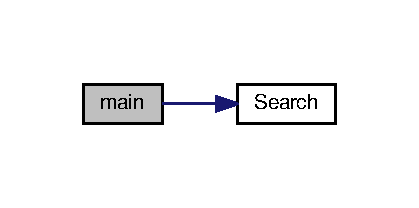
\includegraphics[width=201pt]{Lab3_8cpp_a0ddf1224851353fc92bfbff6f499fa97_cgraph}
\end{center}
\end{figure}


\index{Lab3.\+cpp@{Lab3.\+cpp}!Search@{Search}}
\index{Search@{Search}!Lab3.\+cpp@{Lab3.\+cpp}}
\subsubsection[{\texorpdfstring{Search(void $\ast$arg)}{Search(void *arg)}}]{\setlength{\rightskip}{0pt plus 5cm}void$\ast$ Search (
\begin{DoxyParamCaption}
\item[{void $\ast$}]{arg}
\end{DoxyParamCaption}
)}\hypertarget{Lab3_8cpp_a309dddc4f36d285135261c13128963c1}{}\label{Lab3_8cpp_a309dddc4f36d285135261c13128963c1}

\begin{DoxyCode}
45 \{
46    \hyperlink{structThreadParam}{ThreadParam} * param = (\hyperlink{structThreadParam}{ThreadParam} *) arg;
47    \textcolor{keywordtype}{int} * array = param->\hyperlink{structThreadParam_aec444b4eb12a9a8fea3e8689e149c222}{array};
48    \textcolor{keywordtype}{int} start = param->\hyperlink{structThreadParam_a48b6fa880b0369abac96f8f54bf12e08}{startIndex};
49    \textcolor{keywordtype}{int} end = param->\hyperlink{structThreadParam_a88bf854942e7037fbdd9269b434612d6}{endIndex};
50    \textcolor{keywordtype}{int} value = param->\hyperlink{structThreadParam_a67d5841b5ec120d0265bc55eeb8bac6b}{value};
51    \textcolor{keywordtype}{int} count = 0;
52    \textcolor{keywordtype}{int} pos = 0;
53 
54    cout <<\textcolor{stringliteral}{"Search array["}<<start<<\textcolor{stringliteral}{"..."}<<end<<\textcolor{stringliteral}{"] for value "}<<
55       value<<endl;
56    \textcolor{comment}{//search through designated area for the target number and first position                               
                                                                                                       }
57    \textcolor{keywordflow}{for}(\textcolor{keywordtype}{int} k=start; k<=end; k++)
58    \{
59       \textcolor{keywordflow}{if}(array[k] == value)
60       \{
61          count++;
62          \textcolor{keywordflow}{if}(count == 1)
63             pos = k;
64       \}
65    \}
66    \hyperlink{structThreadReturn}{ThreadReturn} * r = \textcolor{keyword}{new} \hyperlink{structThreadReturn}{ThreadReturn};
67    r->\hyperlink{structThreadReturn_ada06b95a1d8c2688d8f7ff617ca82074}{count} = count;
68    r->\hyperlink{structThreadReturn_acee40ef3ef81baf05c35b71761d7ffad}{pos} = pos;
69    \textcolor{keywordflow}{return} (\textcolor{keywordtype}{void} *)r;
70 \}
\end{DoxyCode}

%--- End generated contents ---

% Index
\backmatter
\newpage
\phantomsection
\clearemptydoublepage
\addcontentsline{toc}{chapter}{Index}
\printindex

\end{document}
